\section{Biaxial mechanical testing simulation}\label{sec:biaxialsimulation}

	A square patch was used to represent the soft tissue. An equivalent of 1 MPa in first Piola-Kirchhoff stress was applied evenly at nodal points along the edge of the patch, with varying direction for the material axis. The deformation within the patch was computed, and the resulting mechanical response was compared to analytical solution of $\Psi_{eff}$ (Eqn. \ref{eqn:finalexponentialmodelformscaled}). No difference in the resulting response was found. 

\begin{figure}[!htbp]
\centering
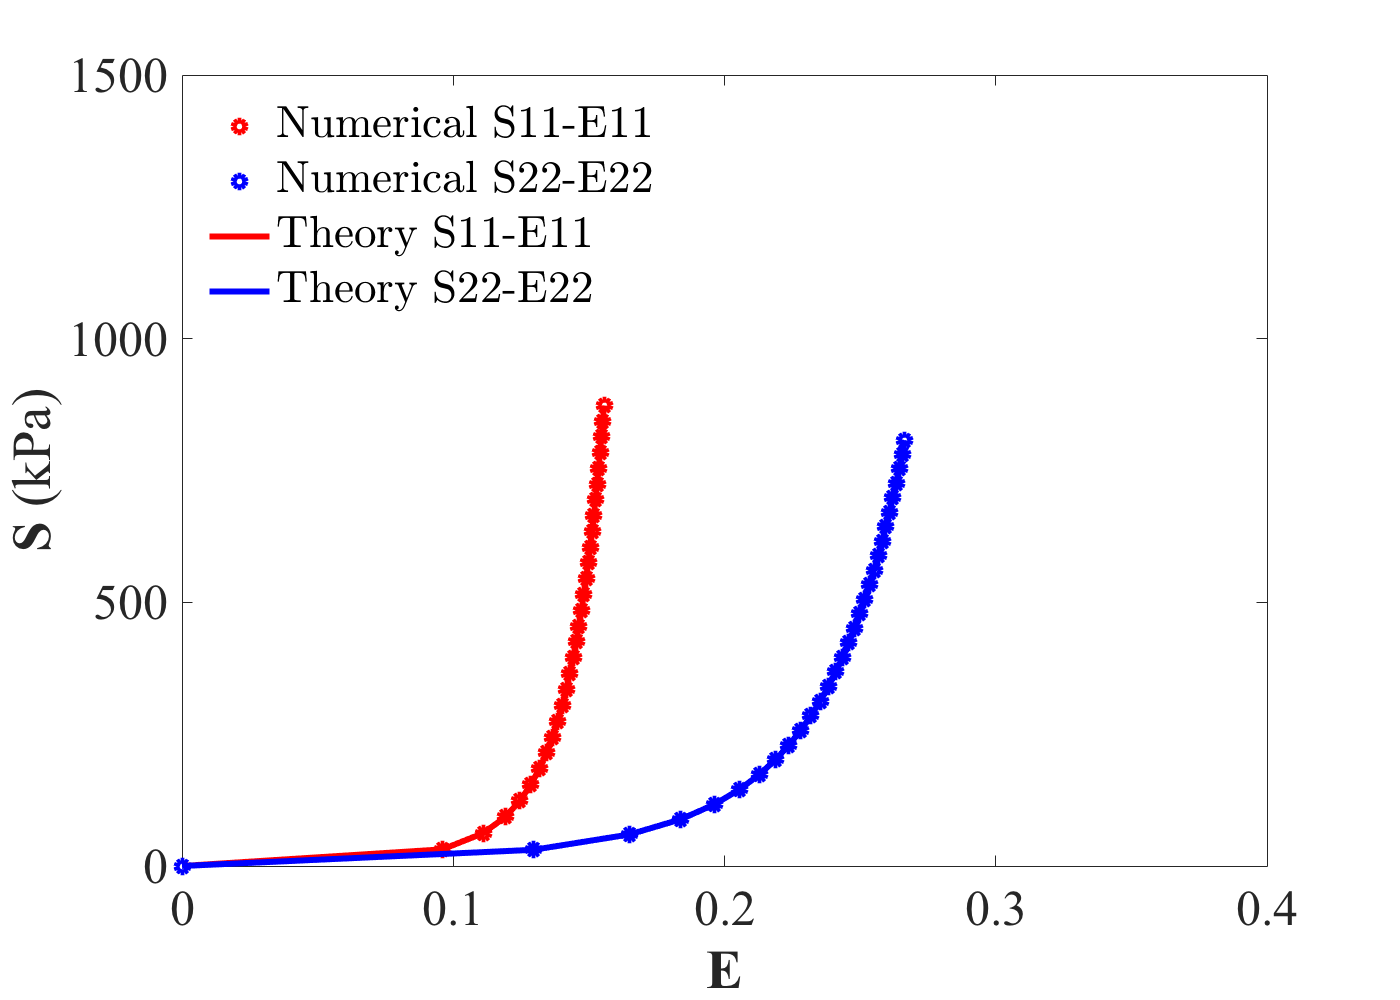
\includegraphics[width=3.25in]{Figures/validation.png}
\caption{Verification and validation of the correct implementation of the constitutive model where predicted Green’s strains from an equibiaxial loading path of a single IGA element compared with the theoretical result demonstrating exact agreement (left).}
\label{fig:biaxvalidation}
\end{figure}